%!TEX root = /Users/ego/Boulot/TKZ/tkz-tab/doc/TKZdoc-tab-main.tex 
% 20 / 02 /2009 v1.00c TKZdoc-tab-valeurs
\section{Valeurs intermédiaires \addbs{tkzTabVal}}
Cette macro permet de placer une valeur sur une flèche de la ligne des variations. Elle doit être employée juste après la commande \tkzcname{tkzTabVar} définissant la ligne de variations sur laquelle on souhaite placer les valeurs intermédiaires. On ne peut placer une valeur que dans un intervalle où la fonction est \tkzname{monotone}. Cette macro permet d'afficher une nouvelle valeur (intermédiaire) dans la première ligne. 

\subsection{Définition de   \addbs{tkzTabVal}}

\begin{NewMacroBox}{tkzTabVal}{\oarg{local options}\{Début\}\{Fin\}\{Position\}\{Antécédent\}\{Image\}}

\begin{tabular}{lllc}
\toprule
\texttt{arguments}   & \texttt{défaut}    & \texttt{définition}                        \\
\midrule
\IargName{tkzTabVal}{Début}     & |no default|  & rang de l'origine de la flèche       \\
\IargName{tkzTabVal}{Fin}       & |no default|  & rang de l'extrémité de la flèche     \\
\IargName{tkzTabVal}{Position}  & |no default|  & nombre décimal entre $0$ et $1$      \\
\IargName{tkzTabVal}{Antécédent}& |no default|  & valeur de l'antécédent si nécessaire \\
\IargName{tkzTabVal}{Image}     & |no default|  & valeur de l'image  si nécessaire     \\
\bottomrule
\end{tabular}

\medskip
\noindent\emph{Ceci mérite quelques commentaires : Il s'agit de savoir sur quelle flèche, on va positionner l'image. \tkzname{Début} et \tkzname{Fin} sont les rangs des valeurs qui déterminent les extrémités de la flèche. \tkzname{Antécédent}  \tkzname{Image} sont les valeurs que l'on veut placer. \tkzname{Position} est    un nombre qui est  obligatoirement compris entre $0$ et $1$. C'est une abscisse en prenant comme origine  \tkzname{Début} et comme extrémité  \tkzname{Fin}.}

\medskip
\begin{tabular}{lllc}
\toprule
\texttt{options}   & \texttt{défaut}    & \texttt{définition}                                      \\
\midrule
\IoptName{tkzTabVal}{draw}    & |true|   & dessin d'une flèche entre l'antécédent et son image     \\
\IoptName{tkzTabVal}{remember}& |lastval|& définit un node personnalisé                            \\
\bottomrule
\end{tabular}

\medskip
\noindent\emph{Si vous  voulez  une flèche entre l'antécédent et l'image, il vous suffit de passer en option  \tkzname{draw}. Si vous voulez référencer le point où se situe l'image alors il faut utiliser l'option \tkzname{remember}.}
\end{NewMacroBox}

\subsubsection{Ajout de valeurs intermédiaires} 

Le premier exemple montre des valeurs remarquables pour la fonction $\ln$. Il s'agit de mettre en évidence des valeurs importantes pour la fonction. La fonction est monotone  entre les valeurs de rang $1$ ($0$) et $2$ ($+\infty$), ainsi les deux premiers arguments sont $1$  et $2$. Les coefficients utilisés pour  \tkzname{Position} sont des nombres \tkzname{décimaux} ici $0.33$ et $0.66$. Les antécédents n'étaient pas présents dans la première ligne aussi leurs valeurs sont passées dans les arguments.

\begin{tkzexample}[code only]
    \tkzTabVal{1}{2}{0.33}{1}{0}
    \tkzTabVal{1}{2}{0.66}{\E}{1}
\end{tkzexample}

\begin{tkzexample}[vbox, small]
\begin{tikzpicture}
\tkzTabInit[lgt=3,espcl=10] {$x$    /1, Signe\\ de $\dfrac{1}{x}$  /1.5,%
                       Variation\\ de $\ln$   /2} {$0$ , $+\infty$}%
    \tkzTabLine{d,+,}%
    \tkzTabVar[color=red]{ D- /  $-\infty$, + /  $+\infty$ }
    \tkzTabVal{1}{2}{0.33}{1}{0}
    \tkzTabVal{1}{2}{0.66}{\E}{1}
\end{tikzpicture}
\end{tkzexample}

\subsubsection{Ajout de valeurs intermédiaires avec une fonction non monotone } 

On ne peut utiliser la macro que sur un intervalle où la fonction est monotone, ici il y a trois valeurs 
\mbox{$0$, $\E$ et $+\infty$}. La fonction est monotone entre les deux premières c'est à dire entre  les valeurs de rang $1$ et $2$ ainsi qu'entre les deux dernières de rang $2$ et $3$.

\begin{tkzexample}[vbox,small]
\begin{tikzpicture}
  \tkzTabInit[espcl=6]{$x$ / 1 , $f'(x)$ / 1, $f(x)$ / 2}
                      {$0$, $\E$ , $+\infty$}%
  \tkzTabLine{d,+,0,-,}%
  \tkzTabVar{D- / $-\infty$, + / $\E$, - / $0$  }%
  \tkzTabVal[draw]{1}{2}{0.6}{$1$}{$\dfrac{1}{\E}$}%
  \tkzTabVal[draw]{2}{3}{0.4}{$\E^2$}{$1$}%
\end{tikzpicture}
\end{tkzexample}

\subsubsection{Ajout de valeurs intermédiaires  avec un palier} 

Il ne faut pas s'arrêter au deuxième antécédent. La fonction est  monotone mais admet un palier. L'option \tkzname{R} permet d'éviter qu'une flèche s'arrête pour $\sqrt\E$. La flèche va donc de la valeur de rang $1$ à la valeur de rang $3$. Le code est donc :
\begin{tkzexample}[code only]
  \tkzTabVal[draw]{1}{3}{0.6}{\E}{$\dfrac{-1}{\E}$} 
\end{tkzexample}

\begin{tkzexample}[vbox,small]
\begin{tikzpicture}
 \tkzTabInit[espcl=6]{$x$/1,$f'(x)$/1, $f(x)$/2}
                     {$0$,$\sqrt\E$,$+\infty$}%
 \tkzTabLine{d,+,0,+,}%
 \tkzTabVar{D-  / $-\infty$,R  /     ,+  / $0$  }
 \tkzTabVal[draw]{1}{3}{0.4}{$1$}{$-\E$}
\end{tikzpicture}
\end{tkzexample}


\subsubsection{Valeurs intermédiaires et plusieurs lignes de variations }
\Iopt{tkzTabVal}{draw}

Les variations de  $f$ et $f'$ sont représentées. Pour $f$ la valeur $1$ n'est pas utilisée, on passe donc du rang $1$ au rang $3$.

\begin{tkzexample}[vbox,small]
\begin{tikzpicture} 
  \tkzTabInit[espcl=6]{$x$/1,$f''(x)$/1,$f'(x)$/3,$f(x)$/3}
  {$0$,$1$,$+\infty$}% 
  \tkzTabLine{d,+,0,-, }%
  \tkzTabVar{-/ $-\infty$ ,+/ ,-/ $-\infty$ }
  \tkzTabVal[draw]{1}{2}{0.3}{$0,3$}{$-2$}
  \tkzTabVal[draw]{2}{3}{0.6}{$4$}{$-1$} 
  \tkzTabVar{+/ $+\infty$,R ,-/ $-1$} 
  \tkzTabVal[draw]{1}{3}{0.6}{$2$}{$0$}
\end{tikzpicture}  
\end{tkzexample}
 
\subsection{Utilisation des options}

\subsubsection{\texttt{\textcolor{red}{draw}} : ajout d'une flèche vers la valeur ajoutée}\Iopt{tkzTabVal}{draw}
L'option a déjà été utilisée dans les exemples précédents, en voici un autre. 

\begin{tkzexample}[vbox,small]
\begin{tikzpicture}
 \tkzTabInit[lgt=3,espcl=10]{$x$                 /1,
                       Signe\\ de $\dfrac{1}{x}$ /2,
                       Variation\\ de $\ln$      /3}
                       {$0$           , $+\infty$  }%
 \tkzTabLine           {d,+           ,            }%
 \tkzTabVar[color=red]{D-/ $-\infty$ , +/$+\infty$}%
 \tkzTabVal[draw]{1}{2}{0.24}{\scriptsize $1-h$}{$<0$}%
 \tkzTabVal[draw]{1}{2}{0.3}{$1$}{$0$}%
 \tkzTabVal[draw]{1}{2}{0.36}{\scriptsize $1+h$}{$>0$}%
 \tkzTabVal[draw]{1}{2}{0.64}{$2,7$}{$<$}%
 \tkzTabVal[draw]{1}{2}{0.7}{$\E$}{$1$}%
 \tkzTabVal[draw]{1}{2}{0.76}{$2,8$}{$>$}%
\end{tikzpicture}
\end{tkzexample}


\subsubsection{\texttt{\textcolor{red}{remember}} : attribuer un nom à  un point ou un node.}
\Iopt{tkzTabVal}{remember}

Cette option permet d'utiliser \tkzcname{tkzTabImaFrom} mais il est possible de récupérer les noms des nodes et de les traiter avec par exemple du code de \TIKZ.

\begin{tkzexample}[code only]
  \draw[opacity=0.4,fill=red!20]  (vb) circle(3ex);
  \draw[opacity=0.4,fill=blue!20]  (vc) circle(3ex);
\end{tkzexample}


\begin{tkzexample}[,small]
  \begin{tikzpicture}
  \tkzTabInit[lgt=3,espcl=6]{ $x$/1,/1,/3,/3 }%
             {  $a$    , $d$    ,$e$}
  \tkzTabLine{  z,+    ,z,-     ,z  } 
  \tkzTabVar  {-/\va  ,+/\vd   , -/  \ve}
  
  \tkzTabVal[draw,remember=vb]{1}{2}{0.333}{$b$}{$0$}
  \tkzTabVal[draw,remember=vc]{1}{2}{0.666}{$c$}{$1$}
  
  \tkzTabVar{-/\va  ,R/   , +/  \ve}
  
  \tkzTabVal[draw]{1}{3}{0.5}{}{$0$}
  
  \draw[opacity=0.4,fill=red!20]  (vb) circle(3ex);
  \draw[opacity=0.4,fill=blue!20]  (vc) circle(3ex);
  \end{tikzpicture}
\end{tkzexample}

\medskip
Il faut remarquer que $b$ et $c$ sont des valeurs intermédiaires car le tableau a été défini avec $a$, $d$ et $e$.
\endinput